% !TeX root = ./pf.tex

%\includeonlyframes{current}

\section*{Dynamic polymorphism}

\begin{frame}[fragile]{Polymorphism}

  \textit{The provision of a single interface to entities of different types}

  \begin{description}
  \item<2-> [static] Based on concepts and templates
    \begin{codeblock}
template<class Iterator, class T>
Iterator std::find(Iterator f, Iterator l, T const& v);

std::vector<int> v\{\ddd\};
auto it = std::find(v.begin(), v.end(), 12);

std::list<Command> l\{\ddd\};
auto it = std::find(l.begin(), l.end(), Command\{"send"\});\end{codeblock}
  \item<3-> [dynamic] Based on inheritance and virtual functions
  \end{description}
\end{frame}

\begin{frame}[fragile]{Inheritance}

  \begin{columns}[T]
    \begin{column}{.4\textwidth}
  \begin{codeblock}{
struct Base \{
  int a;
  Base(int a) : a\{a\} \{\}
  void f();
  int operator()() const;
\};

struct Derived \alert{: Base} \{
  double d;
  Derived(int i, double d)
    : \alert{Base}\{i+1\}, d\{d\} \{\}
  int h() const;
\};

Derived de\{42, 3.14\};
de.d;
de.h();
de.a;   // Base::a
de.f(); // Base::f
de();   // Base::operator()
\uncover<2->{Base* b1 = &de;}
\uncover<3->{Base& b2 = de;}
}\end{codeblock}
   
    \end{column}
    \begin{column}{.6\textwidth}

      \begin{itemize}
      \item A class may be declared as \textit{derived} from one or more
        \textit{base} classes
        \begin{itemize}
        \item A hierarchy can be formed
        \end{itemize}
      \item Members of the base class are also members of the derived class
        \begin{itemize}
        \item Let's ignore access control (\code{private}, \code{public}) for
          the moment
        \end{itemize}
      \item Constructing a \code{Derived} object constructs also the
        corresponding \code{Base} \textit{sub-object}, either explicitly (like
        in this case) or implicitly
      \item<2-> \code{Derived*} can be implicitly converted to \code{Base*}
      \item<3-> A \code{Derived} object can bind to \code{Base\&}
      \end{itemize}
    \end{column}
  \end{columns}

\end{frame}

\begin{frame}[fragile]{Dynamic polymorphism}

  Typical use case: a graphics system of shapes

  \begin{codeblock}

struct Circle \{ // \textit{is a} Shape
  Point c;
  double r;
  void move(Point p);
  Point where() const;
\};

struct Rectangle \{ // \textit{is a} Shape
  Point ul;
  Point lr;
  void move(Point p);
  Point where() const;
\};

std::vector<\textit{Shape}> shapes;                     // I wish I could do this
for (auto const& s : shapes) \{ s.where(); \}    // wish
for (auto& s : shapes) \{ s.move(Point\{1,2\}); \} // wish\end{codeblock}

{\footnotesize Let's ignore access control (\code{private}, \code{public}) for the moment}

\end{frame}

\begin{frame}<trans:0>[fragile]{Dynamic polymorphism \insertcontinuationtext}

  \begin{codeblock}

\uncover<2->{struct Shape \{}\only<2>{ // \alert{base class}}\only<6>{ // \alert{abstract} base class}
\uncover<9->{  \alert<9>{virtual \~Shape();} // no \upquote{= 0} here}
\uncover<6->{  \alert<6>{virtual} Point where() const \alert<6>{= 0};\only<6>{ // \alert{pure virtual function}}}
\uncover<2->{\};}

struct Circle \alt<1>{\{ // \textit{is a} }{: }Shape \uncover<2->{\{}\only<2>{ // \alert{derived class}}
  Point c;
  int r;
  \uncover<9->{\alert<9>{\~Circle();}}
  Point where() const\only<6->{ \alert<6>{override}};
\};

struct Rectangle \alt<1>{\{ // \textit{is a} }{: }Shape \uncover<2->{\{}\only<2>{ // \alert{derived class}}
  Point ul;
  Point lr;
  \uncover<9->{\alert<9>{\~Rectangle();}}
  Point where() const\only<6->{ \alert<6>{override}};
\};

\uncover<3->{\only<-3>{     }\only<4-9>{Shape}\only<8-9>{\alert{*}}\only<10->{\alert<10>{std::unique_ptr<Shape>}} create_shape();\only<3>{ // either a Circle or a Rectangle}}\only<7>{ // \alert<7>{error, cannot instantiate an abstract base class}}\only<8>{ // return \alert<8>{new} Circle/Rectangle}\only<10>{ // use a \textit{smart pointer}}
\uncover<5->{auto s = create_shape();}
\uncover<5->{s\alt<-7>{.}{\alert<8>{->}}where();}\only<5>{ // \alert<5>{error}}
\only<9>{\alert{delete s};}\only<10>{\alert{// automatically deleted at end of scope}}\end{codeblock}
\end{frame}

\begin{frame}<0|trans:1>[fragile]{Dynamic polymorphism \insertcontinuationtext}

  \begin{codeblock}{
struct Shape \{                     // \alert{abstract} base class
  \alert{virtual} Point where() const \alert{= 0}; // \alert{pure virtual} function
  \alert{virtual} \~Shape();                // virtual dtor; no \upquote{= 0} here
\};

struct Circle : Shape \{ // derived class
  Point c;
  int r;
  Point where() const \alert{override};
\};

struct Rectangle : Shape \{ // derived class
  Point ul;
  Point lr;
  Point where() const \alert{override};
\};

Shape\alert{*} create_shape();   // return \alert{new} Circle/Rectangle
auto s = create_shape();
s->where();
delete s;                // better use a smart pointer
}\end{codeblock}

\end{frame}

\begin{frame}{Dynamic polymorphism \insertcontinuationtext}

  \begin{itemize}
  \item<1-> A non-static member function (i.e. a method) is a \textbf{virtual}
    function if it is first declared with the keyword \code{virtual} or if it
    \textbf{override}s a virtual member function declared in a base class
  \item<1-> A class with a virtual member function is called a
    \textbf{polymorphic} class.
  \item<2-> Virtual functions support \textbf{dynamic binding} and
    \textbf{object-oriented programming}
    \begin{itemize}
    \item A call to a virtual function made through a pointer/reference to a
      base class is dispatched to the corresponding function of the actual
      derived class object behind that pointer/reference
    \end{itemize}
  \item<2-> Overridden functions must have the same signature
    \begin{itemize}
    \item Beware of member function hiding
    \end{itemize}
  \end{itemize}

\end{frame}


\begin{frame}{Dynamic polymorphism \insertcontinuationtext}

  \begin{itemize}
  \item A virtual function is \textbf{pure} if its declaration ends with
    \code{= 0}
    \begin{itemize}
    \item A pure virtual function cannot be defined (i.e. have an
      implementation) -- with one exception (see later)
    \end{itemize}
  \item A class is \textbf{abstract} if it has at least one pure virtual
    function
    \begin{itemize}
    \item No objects of an abstract class can be created
    \item An abstract class is typically used to represent an \textit{interface} 
    \end{itemize}
  \end{itemize}

\end{frame}

\begin{frame}[fragile]{Dynamic polymorphism \insertcontinuationtext}

  \begin{codeblock}{
struct Base \{
  virtual void f(int) = 0;
\};

struct Derived : Base \{
  void f(int) override \{\ddd\}
\};

\uncover<2->{Base b;                 // error}
\uncover<3->{Base* b1 = new Derived; // ok, owning pointer, remember to delete}
\uncover<3->{b1->f(0);               // calls Derived::f}
\uncover<4->{Derived d;              // ok}
\uncover<4->{Base* b2 = &d           // ok, non-owning pointer, don\textquotesingle{}t delete}
\uncover<4->{b2->f(0);               // calls Derived::f}
\uncover<5->{Base& b3 = d;           // ok}
\uncover<5->{b3.f(0);                // calls Derived::f}
}\end{codeblock}

\end{frame}

\begin{frame}<trans:0>[fragile]{Mixing interface and implementation}

  \begin{codeblock}
struct Shape \{
  \uncover<2->{\alert<2>{Point p;
  Shape(Point p) : p\{p\} \{\}}}
  virtual \~Shape();
  virtual Point where() const \only<-2>{= 0;}\only<3->{\alert<3>{\{ return p; \}} // \alert<3>{default implementation}}
\};

struct Circle : Shape \{
  \uncover<1>{\alert{Point c;}}
  int r;
  Circle(Point p, double d) : \alt<1>{c\{p\}}{\alert<2>{Shape\{p\}}}, r\{d\} \{\}
  \~Circle();
  \alt<-2>{Point where() const override \{ return \alt<1>{c}{p}; \}}{\alert<3>{// where() is inherited from Shape}}\only<2>{ // \alert{p is inherited}}
\};

struct Rectangle : Shape \{
  \uncover<1>{\alert{Point ul;}}
  Point lr;
  Rectangle(Point p1, Point p2) : \alt<1>{ul\{p1\}}{\alert<2>{Shape\{p1\}}}, lr\{p2\} \{\}
  \~Rectangle();
  Point where() const override \{ return (\temporal<2,3>{ul}{p}{\alert<4>{Shape::where()}} + lr) / 2; \}\only<2>{ // \alert{p is inherited}}
\};\end{codeblock}

  \uncover<5>{Not recommended, especially for data members}

\end{frame}

\begin{frame}<0|trans:1>[fragile]{Mixing interface and implementation}

  \begin{codeblock}{
struct Shape \{
  \alert{Point p;}
  Shape(Point p) : p\{p\} \{\}
  virtual \~Shape();
  virtual Point where() const \{ return p; \} // \alert{not pure; default implementation}
\};

struct Circle : Shape \{
  int r;
  Circle(Point p, double d) : \alert{Shape\{p\}}, r\{d\} \{\}
  // where() implementation is inherited from Shape
\};

struct Rectangle : Shape \{
  Point lr;
  Rectangle(Point p1, Point p2) : \alert{Shape\{p1\}}, lr\{p2\} \{\}
  Point where() const override \{ return (\alert{p} + lr) / 2; \} // \alert{p is inherited}
\};
}\end{codeblock}

  \uncover<5>{Not recommended, especially for data members}

\end{frame}

\begin{frame}{Example: SFML}
% @startuml
% interface sf::Drawable {
%   {abstract} void draw()
% }
% class sf::Transformable {
%   void move()
%   .. private ..
%   Point m_position
% }

% sf::Shape <|-- sf::RectangleShape
% sf::Shape <|-- sf::CircleShape
% sf::Shape <|-- sf::ConvexShape
% sf::Transformable <|-- sf::Shape
% class sf::Shape implements sf::Drawable
% @enduml
  \centering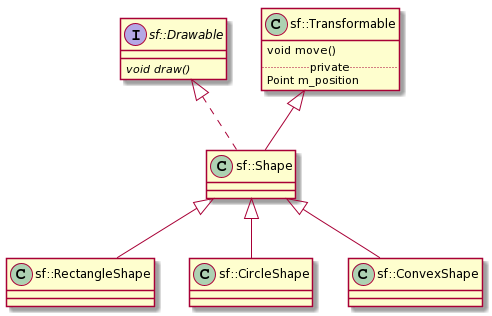
\includegraphics[width=\textwidth]{images/sfml-shapes}
\end{frame}

\begin{frame}[fragile]{An example from the Standard Libary: I/O streams}
% @startuml
% class std::basic_ios<CharT, Traits> extends std::ios_base
% class std::basic_ostream<CharT, Traits> extends std::basic_ios
% class std::basic_istream<CharT, Traits> extends std::basic_ios
% class std::basic_iostream<CharT, Traits> extends std::basic_istream
% class std::basic_iostream<CharT, Traits> extends std::basic_ostream

% class std::basic_ostringstream<CharT, Traits> extends std::basic_ostream
% class std::basic_ofstream<CharT, Traits> extends std::basic_ostream

% class std::basic_stringstream<CharT, Traits> extends std::basic_iostream
% class std::basic_fstream<CharT, Traits> extends std::basic_iostream

% class std::basic_istringstream<CharT, Traits> extends std::basic_istream
% class std::basic_ifstream<CharT, Traits> extends std::basic_istream
% @enduml
  \centering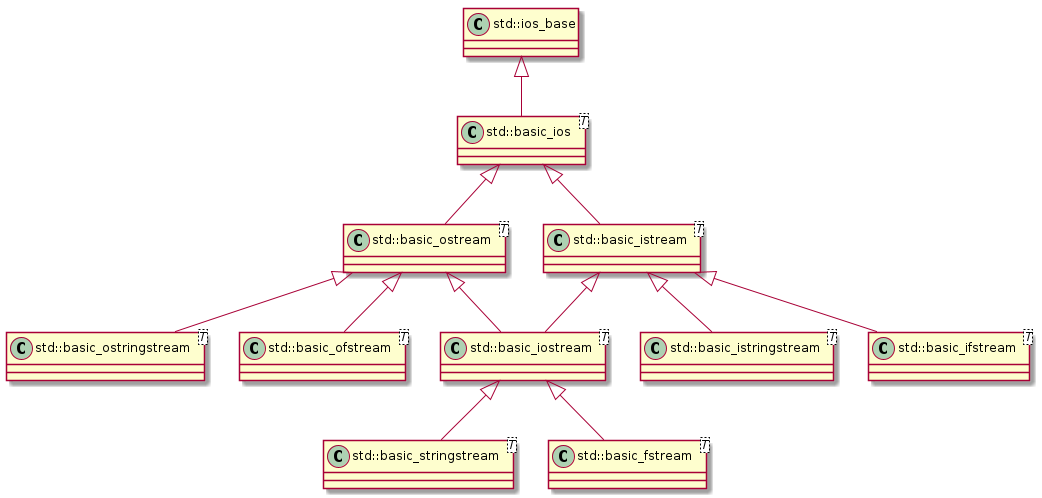
\includegraphics[width=\textwidth]{images/iostream}
  \begin{codeblock}<2->{\tiny
namespace std \{
  using istream = basic_istream<char>;
  using ostream = basic_ostream<char>;
  using istringstream = basic_istringstream<char>;
  using ostringstream = basic_ostringstream<char>;
  using ifstream = basic_ifstream<char>;
  using ofstream = basic_ofstream<char>;
  \ddd
  \uncover<3->{istream cin;
  ostream cout;}
\}}\end{codeblock}
\end{frame}

\begin{frame}{I/O Streams}

  \begin{itemize}
  \item C++ provides an Input/Output library based on the concept of \textit{streams}, which abstract input/ouput devices
  \item \code{std::cin} and \code{std::cout} are streams attached to the
    standard input and output of the program (typically attached to the
    terminal)
  \item Other stream classes allow I/O from/to files and strings
  \item Since they are part of a polymorphic hierarchy these objects can be
    passed to functions implemented in terms of the base class
    \begin{itemize}
    \item For example the \textit{streaming} operators \code{<<} and \code{>>}
    \end{itemize}
  \end{itemize}
\end{frame}

\begin{frame}[fragile]{File I/O}

  \begin{codeblock}
std::ifstream is\{"/tmp/in"\};  // open /tmp/in for reading
std::ofstream os\{"/tmp/out"\}; // open /tmp/out for writing
if (!is || !os) \{
  // manage error
\}
double d;
while (is \alert{>>} d) \{
  os \alert{<<} std::setw(12) \alert{<<} d * 2 \alert{<<} \bslashn{};
\}\end{codeblock}

  \begin{itemize}
  \item \code{fstream} constructor opens the file, destructor closes it
  \item There are explicit \code{open} and \code{close} methods
  \item Many other operations/options (mostly inherited)
  \end{itemize}

\end{frame}

\begin{frame}[fragile]{String I/O}

  \begin{codeblock}
std::istringstream is\{"12. 14. -42."\};
std::ostringstream os;

double d;
while (is \alert{>>} d) \{
  os \alert{<<} std::setw(12) \alert{<<} d * 2 \alert{<<} \bslashn{};
\}

std::cout << os.str();
// "          24\\n          28\\n         -84\\n"\end{codeblock}

  \begin{itemize}
  \item \code{stringstream} constructor possibly allocates memory, destructor
    deallocates
  \item The \code{str} method can be used to get/set the contents of the
    \code{stringstream}
  \item Many other operations/options (mostly inherited)
  \end{itemize}
\end{frame}

\begin{frame}[fragile]{\code{operator<<}}

  \begin{itemize}
  \item \code{operator<<} is usually implemented as a free function
    \begin{itemize}
    \item Note that the object we want to stream is the second parameter
    \end{itemize}

  \begin{codeblock}
class Complex \{
  double r;
  double i;
 public:
  double real() const;
  double imag() const;
  \ddd
\};

inline std::ostream& operator<<(std::ostream& os, Complex const& c)
\{
  os << \upquote{(} << c.real() << \upquote{,} << c.imag() << \upquote{)};
  return os;
\}\end{codeblock}

  \item To be more general, it should actually be a function template and
    accept/return \code{std::basic_ostream<\ddd>}
  \end{itemize}
\end{frame}

\begin{frame}[fragile]{\code{friend} functions}

  \begin{itemize}
  \item Sometimes a free function (e.g. \code{operator<<} needs private data
    that are not exposed (or not exposed efficiently) via the public interface
  \item In that case it can be implemented as a \code{friend} free function

    \begin{codeblock}
class Complex \{
  double r; double i;
 public:
  \alert{friend} std::ostream& operator<<(std::ostream& os, Complex const& c) \{
    os << \upquote{(} << c.\alert{r} << \upquote{,} << c.\alert{i} << \upquote{)};
    return os;
  \}
  \ddd
\};\end{codeblock}

  \item Note how the function, being defined inside the class definition, is
    automatically \code{inline}
  \item It can be just declared inside the class definition and be defined
    outside, even in another file
  \item \textit{friendship} has a much broader usage than shown here
    \begin{itemize}
    \item E.g. a whole class can be \code{friend} of another
    \end{itemize}
  \end{itemize}
\end{frame}

\begin{frame}{Another example from the Standard Library: Exceptions}
% @startuml
% class std::exception {
%   what()
% }
% class std::system_error {
%   code()
% }
% class std::filesystem_error {
%   path1()
%   path2()
% }
% class std::runtime_error extends std::exception
% class std::bad_cast extends std::exception
% class std::bad_alloc extends std::exception
% class std::system_error extends std::runtime_error
% class std::regex_error extends std::runtime_error
% class std::range_error extends std::runtime_error
% class std::filesystem::filesystem_error extends std::system_error
% @enduml
  \centering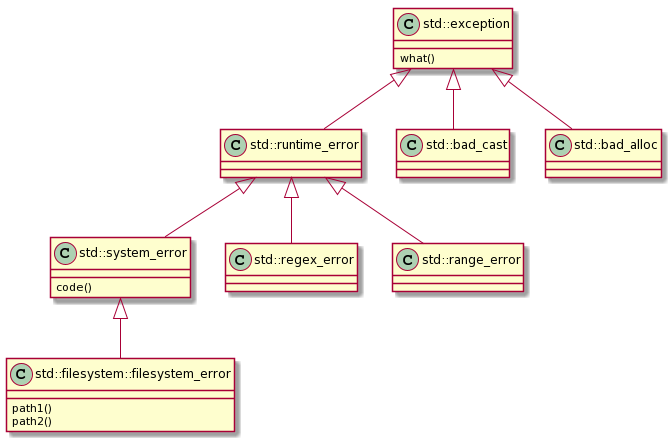
\includegraphics[width=\textwidth]{images/exceptions}
  Note: the hierarchy is incomplete
\end{frame}

\begin{frame}[fragile]{Multiple exception-catch clauses}

  \begin{itemize}
  \item A \code{try}-block can have multiple catch clauses
  \item The first that matches the type of the exception is chosen
  \item The order is important: put the more specific ones first
  \end{itemize}
  \begin{codeblock}{\tiny
auto read_from(std::filesystem::path const& p) \{
  std::ifstream is(p);
  if (!is) \{
    throw std::filesystem::filesystem_error\{
      "read_from", p, std::make_error_code(std::errc::invalid_argument)
    \};
  \}
  \ddd
\}

int main() \{
  try \{
    read_from("/tmp/data");
    \ddd
  \} catch (std::filesystem::filesystem_error const& e) \{
    std::cerr << e.path1(); return EXIT_FAILURE;
  \} catch (std::exception const& e) \{
    std::cerr << e.what(); return EXIT_FAILURE;
  \} catch (...) \{ \alert{// it\textquotesingle{}s really three dots!}
    std::cerr << "unknown exception"; return EXIT_FAILURE;
  \}
\}}\end{codeblock}
\end{frame}

\begin{frame}[fragile]{Overriding vs hiding}

  \begin{codeblock}{
struct Base \{
  virtual \alert{void f(int)};
\};

struct Derived : Base \{
  \alert{void f(int)}; // overriding, virtuality is "inherited"
\};

Derived d;
Base& b = d;
b.f(1);          // call Derived::f(int)
}\end{codeblock}

  \begin{itemize}
  \item A virtual function should specify exactly one of \code{virtual},
    \code{override}, or \code{final}
  \item A \code{final} virtual function cannot be overridden in a derived class
  \item A class can be declared \code{final} and cannot be derived from
    \begin{codeblock}{
struct Derived final \{ \ddd \};
}\end{codeblock}
  \end{itemize}

\end{frame}

\begin{frame}[fragile]{Overriding vs hiding \insertcontinuationtext}

  \begin{codeblock}{
struct Base
\{
  virtual void f(\alert{int});
\};

struct Derived : Base
\{
  virtual void f(\alert{unsigned}); \uncover<4->{// this is another function}\uncover<7->{, hiding Base::f}
\};

\uncover<2->{Derived d;
Base& b = d;}
\uncover<3->{b.f(1);}\uncover<4->{          // call Base::f(int)}
\uncover<5->{b.f(1U);}\uncover<6->{         // call Base::f(int)}
\uncover<7->{d.f(1);          // call Derived::f(unsigned)}
\uncover<7->{d.f(1U);         // call Derived::f(unsigned)}
}\end{codeblock}

  \begin{itemize}
  \item<9-> Virtual functions should specify exactly one of \code{virtual}, 
    \code{override}, or \code{final}
  \item<9-> Specifying \code{override} (or \code{final}) would have caused
    a compilation error
  \end{itemize}

\end{frame}

\begin{frame}[fragile]{Overriding vs hiding \insertcontinuationtext}

  \begin{codeblock}{
struct Base
\{
    virtual void f(int) \alert{const};
\};

struct Derived : Base
\{
  virtual void f(int); \uncover<3->{// this is another function, hiding Base::f}
\};

\uncover<2->{Derived d;
Base& b = d;
b.f(1);}\uncover<3->{          // call Base::f(int) const}
}\end{codeblock}

  \begin{itemize}
  \item<4-> Virtual functions should specify exactly one of \code{virtual}, 
    \code{override}, or \code{final}
  \item<4-> Specifying \code{override} (or \code{final}) would have caused
    a compilation error
  \end{itemize}

\end{frame}

\begin{frame}[fragile]{Slicing}

  A base class without pure virtual functions is not abstract any more
  \begin{itemize}
  \item<2-> It can be instantiated
  \item<3-> It can be copied
    \begin{itemize}
    \item unless precautions are taken, e.g. copy/move operations are \code{delete}d
    \end{itemize}
  \end{itemize}

  \begin{codeblock}<1->{
struct Shape
\{
  Point p;
  Shape(Point p): p\{p\} \{\}
  virtual ~Shape() = default;
  virtual Point where() const \{ return p; \}
\};

struct Rectangle : Shape \{\ddd\};

\uncover<2->{Shape s;\only<2>{ // \alert{desirable?}}}
\uncover<3->{Shape s2 = s1;\only<3>{ // \alert{desirable?}}}
\uncover<4->{Rectangle rect\{\ddd\};
Shape s = rect;\only<4>{ // \alert{desirable??}}}}\end{codeblock}
\end{frame}

\begin{frame}[fragile]{Slicing \insertcontinuationtext}
  \begin{codeblock}{
\uncover<2->{void process1(\alert<3>{Shape&} shape)\only<3>{ // by reference}
\{
  \ddd shape.where() \ddd\only<4->{ // Point\{2., 4.\}}
\}}

\uncover<5->{void process2(\alert<6>{Shape} shape)\only<6>{ // by value}
\{
  \ddd shape.where() \ddd\only<7->{ // Point\{1., 7.\}}
\}}

\uncover<1->{auto rect = Rectangle\{Point\{1., 7.\}, Point\{3., 1.\}\};}
\uncover<2->{process1(rect);}
\uncover<5->{process2(rect);}
}\end{codeblock}

  \begin{itemize}
  \item<8-> When an object \code{obj} of a derived class is passed to a function
    that takes a parameter of a base class \textbf{by value}, only the base class
    sub-object of \code{obj} is passed to the function
  \end{itemize}

\end{frame}

\begin{frame}[fragile]{Keeping the base class abstract}

  \begin{itemize}
  \item It's good practice to keep base classes abstract
  \item A base class without pure virtual functions is not abstract any more
  \item<2-> To prevent this, declare the destructor as pure virtual
  \item<3-> Yet the destructor needs to be defined
    \begin{itemize}
    \item So that derived classes are properly destroyed
    \end{itemize}
  \end{itemize}

  \begin{codeblock}
struct Shape \{
  Point ul;
  Shape(Point p): p\{p\} \{\}
  virtual ~Shape()\only<2->{\alert<2>{ = 0}};
  virtual Point where() const; // non-pure virtual function
\};
\uncover<3->{inline Shape::~Shape() = default; // or any other implementation}

Shape s; // \alt<1>{\alert{not really desirable}}{\alert<2>{error}}
  \end{codeblock}
\end{frame}

\begin{frame}{Access control}
  A member of a class can be
  \begin{description}
  \item [\code{public}] Its name can be used \textbf{anywhere} without access
    restriction
  \item [\code{private}] Its name can be used \textbf{only by members} and friends of the
    class in which it is declared
  \item [\code{protected}] Its name can be used only \textbf{by members} and
    friends of the class in which it is declared, \textbf{by classes derived}
    from that class, and by their friends
  \end{description}
\end{frame}

\begin{frame}[fragile]{Accessibility through derivation}

  \begin{codeblock}{
class Base \{
 private:
  \ddd
 protected:
  \ddd
 public:
  \ddd
\};

class Derived : \alert{public}\uncover<2->{|\alert{private}}\uncover<3->{|\alert{protected}} Base \{\};
}\end{codeblock}

  Derivation itself can be
  \begin{description}
    \item [\code{public}] \code{public} in B $\rightarrow$ \code{public} in D\\
      \code{protected} in B $\rightarrow$ \code{protected} in D
      \begin{itemize}
      \item Sub-typing (\textit{is-a} relationship)
      \item This is the one you should use
      \end{itemize}
    \item<2-> [\code{private}] \code{public} or \code{protected} in B
      $\rightarrow$ \code{private} in D
      \begin{itemize}
      \item Implementation inheritance
      \end{itemize}
    \item<3-> [\code{protected}] \code{public} or \code{protected} in B
      $\rightarrow$ \code{protected} in D
      \begin{itemize}
      \item Rarely, if ever, used
      \end{itemize}
  \end{description}
\end{frame}

\begin{frame}<trans:0>[fragile]{\code{protected} access}
  \begin{codeblock}
class Shape \{
 \only<5-6>{\alert<5>{protected}:}\only<7->{\alert{private:}}
  Point p;
\uncover<2->{ \alert<2>{public}:}
  Shape(Point p) : p\{p\} \{\}
  virtual ~Shape() = default;
  virtual Point \alert<6>{where}() const \{ return p; \}
  virtual double area() const = 0;
\};

class Rectangle : \alert<1>{public} Shape \{\only<1>{ // \alert{is-a}}
\uncover<4->{ \alert<4>{private}:}
  Point lr;
\uncover<2->{ \alert<2>{public}:}
  Rectangle(Point p1, Point p2) : Shape\{p1\}, lr\{r\} \{\}
  ~Rectangle();
  double area() const override \{ \ddd \uncover<3->{abs(\only<3-5>{\alert{p}}\only<6->{\alert<6>{where()}}.x - \alert<3-5>{lr}.x)} \ddd \}
\};\end{codeblock}

  \uncover<8->{\begin{itemize}
  \item \code{protected} and \code{public} members represent an interface
  \item Data members are a poor interface, keep them private
  \end{itemize}}

\end{frame}

\begin{frame}<0|trans:1>[fragile]{\code{protected} access}
  \begin{codeblock}{
class Shape \{
 \alert{protected}:
  Point p;
 public:
  Shape(Point p) : p\{p\} \{\}
  virtual ~Shape() = default;
  virtual Point where() const \{ return p; \}
  virtual double area() const = 0;
\};

class Rectangle : public Shape \{ // is-a
 private:
  Point lr;
 public:
  Rectangle(Point p1, Point p2) : Shape\{p1\}, lr\{r\} \{\}
  double area() const override \{ \ddd std::abs(\alert{p}.x - lr.x) \ddd \}
\};
}\end{codeblock}

  \begin{itemize}[<8->]
  \item \code{protected} and \code{public} members represent an interface
  \item Data members are a poor interface, keep them private
  \end{itemize}

\end{frame}

\begin{frame}[fragile]{Structural inheritance}

  \begin{itemize}
  \item Inheritance is applicable also in non-polymorphic situations
  \item To reuse and possibly extend the implementation and the interface of a
    class
  \item A way to create a distinct type with the same implementation and
    interface of another
  \item<5-> Consider composition, i.e. a member, or private inheritance
  \end{itemize}

  \begin{codeblock}<2->{
class Vector : public std::vector<int> \{
  using std::vector<int>::vector; // inherit constructors
\};

\uncover<3->{void process(std::vector<int>&); // #1
void process(Vector&);           // #2}
\uncover<4->{void signal(std::vector<int>&);  // #3}

\uncover<3->{std::vector<int> v1\{\ddd\};
Vector v2\{\ddd\};            // all std::vector ctors are available
process(v1);              // call #1
process(v2);              // call #2}
\uncover<4->{signal(v2);               // call #3}}\end{codeblock}

\end{frame}

\begin{frame}[fragile]{Destruction and inheritance}
  \begin{itemize}
  \item In case of polymorphic inheritance, the destructor of a base class
    should be
    \begin{itemize}
    \item \code{public} and \code{virtual}, or
    \item \code{protected} and non-\code{virtual}
    \end{itemize}
  \item<2-> In case of structural inheritance, don't delete through a
    pointer to the base class
  \end{itemize}

    \begin{codeblock}<2->{
class Vector : public std::vector<int> \{\};

\uncover<3->{Vector v;                         // ok}

\uncover<4->{Vector* pv = new Vector;}
\uncover<4->{delete pv;                        // ok}

\uncover<5->{std::vector<int>* ps = new Vector;}
\uncover<5->{delete ps;                        // undefined behavior}}\end{codeblock}

\end{frame}

\begin{frame}[fragile]{Copying/moving and inheritance}
  \begin{itemize}
  \item Dynamic polymorphism and value semantics don't play well together
    \begin{itemize}
    \item See slicing
    \end{itemize}

  \item The copy/move operations of a base class shouldn't be publicly
    accessible, but they need to be accessible to a derived class
    \begin{itemize}
    \item Declare them \code{protected}
    \end{itemize}

    \begin{codeblock}
class Base
\{
  \ddd
 protected:
  Base(Base const&);
  Base& operator=(Base const&);
  Base(Base&&);
  Base& operator=(Base&&);
 public:
  \ddd
\};\end{codeblock}
  \end{itemize}
\end{frame}

\begin{frame}[fragile]{Copying/moving and inheritance \insertcontinuationtext}

  \begin{itemize}
  \item If you need some form of \textit{deep} copy, consider providing a
    virtual \textit{clone} operation

    \begin{codeblock}
class Base
\{
 public:
  virtual Base* clone() const = 0;
\};

class Derived: public Base
\{
 public:
  Derived* clone() const override
  \{
    return new Derived\{*this\}; // call the copy ctor of Derived
  \}
\};\end{codeblock}

  \item Note the return type: an overridden function can return a derived class
    \begin{itemize}
    \item \textit{co-variant} return type
    \end{itemize}
  \end{itemize}

\end{frame}
